\section{Lektion 05-04-2018}

\begin{enumerate}
	\item Højttaler i kabinet
	\item Åben baffel
	\item Lukket kabinet
	\item Basreflex
	\item Slavebas
\end{enumerate}

\begin{mdframed}[style=exampledefault]
	\begin{itemize}
		\item \textbf{Pensum:} 
		\begin{enumerate}
			\item Elektroakustik, TAS,  p. 42-65
		\end{enumerate}
		\item \textbf{Opgaver:} 
		\begin{enumerate}
			\item Lyd og Akustik - Lektion 8 - opgaver og øvelser
		\end{enumerate}
	\end{itemize}
\end{mdframed}

\subsection{Åben baffel}

\subsubsection{Akustisk kortslutning}
\begin{itemize}
	\item Et overtryk på den ene side af membranen vil udligne det tilsvarende undertryk på den anden side.
	\item Ved gengivelse af dybe toner skal lydtrykket fra de to sider af membranen derfor holdes adskilt.
	\item Med et hul i en plade (en baffel) forsinkes og
	dæmpes trykbølgen fra bagsiden.
	\item Herved opstår kun en delvis udslukning af lyden.
\end{itemize}

\begin{figure} [H]
	\centering
	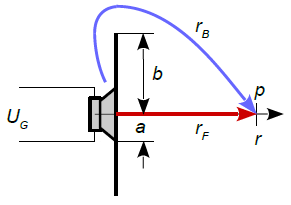
\includegraphics[width=0.5\linewidth]{graphics/53.png}
	\caption{Akustisk kortslutning. \href{http://www.torean.dk/artikel/Elektroakustik.pdf}{(Elektroakustik, TAS)}}
	\label{fig:53}
\end{figure}

\begin{itemize}
	\item Det resulterende lydtryk i afstanden rF beregnes som differensen mellem de to lydtryk.
\end{itemize}

\begin{equation}
p = \dfrac{\rho}{r_F}\dfrac{Bl S_D}{2\pi M_{MS}}\dfrac{U_G}{R_E}\left[1-\dfrac{r_F}{r_B}D(ka)\exp(-jk(r_B-r_F))\right]
\end{equation}


\begin{itemize}
	\item Under	grænsefrekvensen $f_B$ aftager lydtrykket med 6 dB/oktav.
	\item Under højttalerens resonans $f_S$ øges hældningen til 18 dB/oktav. \item Ved høje frekvenser opstår interferens på grund af den skiftende
	fase for bagsidens signal.
	\item Grænsefrekvens $(\lambda/4)$ ved meget stor afstand til mikrofonen.
	\begin{itemize}
		\item Cirkulær baffel med radius $b$.
	\end{itemize}
\end{itemize}

\begin{equation}
f_B=\dfrac{c}{4b}
\end{equation}

\subsubsection{Diffraktion}
\begin{itemize}
	\item Lyden kan ikke uden videre bøjes omkring et skarpt hjørne. 
	\item En kantrefleksion vil	skabe interferens på samme måde som trykbølgen fra bagsiden af højttaleren.
	\item Efter den direkte lyds impuls kommer et svagere og inverteret ekko med en tidsforskel givet ved afstanden fra højttaleren til kanten.
	\item Refleksionskoefficient $R$.
	\begin{itemize}
		\item $R_{Kasse} =−0.33$
		\item $R_{Plade} =−0.50$
	\end{itemize}
\end{itemize}

\begin{figure} [H]
	\centering
	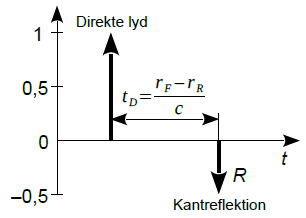
\includegraphics[width=0.5\linewidth]{graphics/54.png}
	\caption{Impulsresponsen for en cirkulær baffel med en punktlydkilde i centrum. \href{http://www.torean.dk/artikel/Elektroakustik.pdf}{(Elektroakustik, TAS)}}
	\label{fig:54}
\end{figure}

\begin{itemize}
	\item Diffraktionen kan beregnes på samme måde som for den akustiske kortslutning ved at addere det direkte bidrag med kantreflektionen.
	\item Det negative fortegn svarer til en subtraktion af det dæmpede og forsinkede ekko fra det direkte signal fra fronten.
\end{itemize}

\begin{equation}
p = \dfrac{\rho}{r_F}\dfrac{Bl S_D}{2\pi M_{MS}}\dfrac{U_G}{R_E}\left[1-\dfrac{r_F}{2r_R}D(ka)\exp(-jk(r_R-r_F))\right]
\end{equation}

\begin{figure} [H]
	\centering
	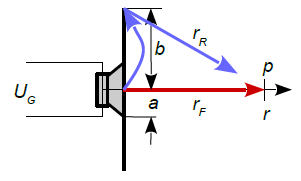
\includegraphics[width=0.5\linewidth]{graphics/55.png}
	\caption{Diffraktion for en cirkulær baffel med radius $b$ og en punktformet lydkilde i centrum. \href{http://www.torean.dk/artikel/Elektroakustik.pdf}{(Elektroakustik, TAS)}}
	\label{fig:55}
\end{figure}

\subsection{Lukket kabinet}
\begin{itemize}
	\item Eliminere udstrålingen fra bagsiden ved at montere højttaleren i et lukket kabinet for effektivt at holde de to sider adskilt.
	\item Den indespærrede luftvolumen $V_B$ udgør en eftergivelighed $C_{AB}$ som	belaster membranens bagside.
	\item En vigtig specifikation for en højttaler er dens ækvivalente volumen $V_{AS}$.
	\item En højttaler med resonansen \SI{50}{\hertz} monteres i et kabinet med samme volumen som $V_{AS}$ specifikationen vil resonansen hæves 1.4
	gange til \SI{70}{\hertz}.
\end{itemize}

\begin{figure} [H]
	\centering
	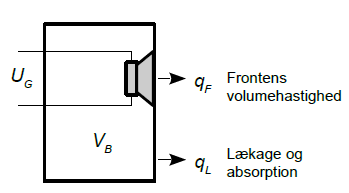
\includegraphics[width=0.5\linewidth]{graphics/59.png}
	\caption{Lukket kabinet. \href{http://www.torean.dk/artikel/Elektroakustik.pdf}{(Elektroakustik, TAS)}}
	\label{fig:59}
\end{figure}
\begin{itemize}
	\item Det resulterende lydtryk for et lukket kabinet.
\end{itemize}
\begin{figure} [H]
	\centering
	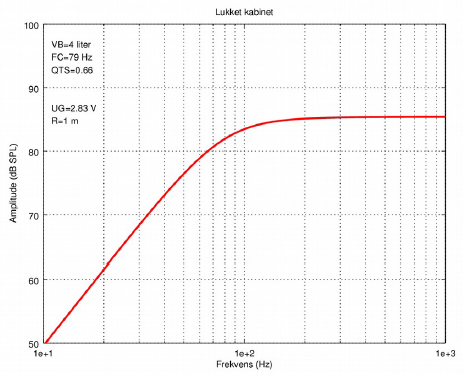
\includegraphics[width=0.75\linewidth]{graphics/58.png}
	\caption{Lukket kabinet. \href{http://www.torean.dk/artikel/Elektroakustik.pdf}{(Elektroakustik, TAS)}}
	\label{fig:58}
\end{figure}


\subsection{Basreflex}
\begin{itemize}
	\item Udnyttelse af effekten fra højttalerens bagside til at støtte basgengivelsen i et mindre frekvensområde ved et såkaldt ventileret kabinet.
	\item Massen af luften i porten danner en resonans	med det indespærrede luftvolumen.
	\item Massen af luftproppen i porten beregnes som massefylden af luft $\rho_0$ gange med luftvoluminet der er arealet af porten $S_P$ ganget med længden af porten $L_P$.
	\item Den omregnes til akustisk masse $M_{AP}$ ved division med $S_P$ kvadreret
\end{itemize}

\begin{equation}
M_{AP}=\dfrac{\rho_0}{S_P}(L_p+1.5\sqrt{\frac{S_P}{\pi}})
\end{equation}

\begin{itemize}
	\item $\rho_0 = \SI{1.18}{\kilogram/\meter\cubic}$
\end{itemize}

\begin{figure} [H]
	\centering
	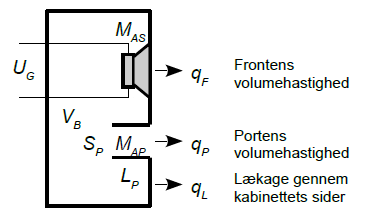
\includegraphics[width=0.5\linewidth]{graphics/56.png}
	\caption{Et basreflex kabinet inkluderer en port. \href{http://www.torean.dk/artikel/Elektroakustik.pdf}{(Elektroakustik, TAS)}}
	\label{fig:56}
\end{figure}
\begin{itemize}
	\item Rød kurve er det resulterende lydtryk.
	\item Grøn kurve er	lydtrykket fra højttalerenheden.
	\item Blå kurve viser hvor meget port står for.
\end{itemize}

\begin{figure} [H]
	\centering
	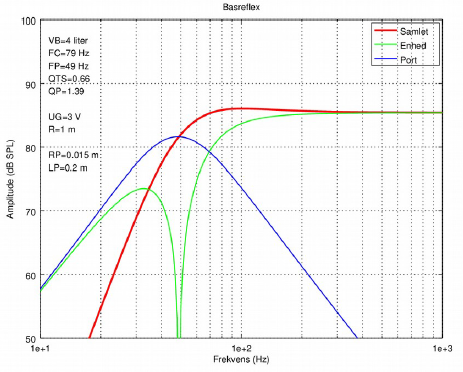
\includegraphics[width=0.75\linewidth]{graphics/60.png}
	\caption{basreflex kabinet. \href{http://www.torean.dk/artikel/Elektroakustik.pdf}{(Elektroakustik, TAS)}}
	\label{fig:60}
\end{figure}

\subsection{Passiv slave}
\begin{itemize}
	\item Erstatter porten med en passiv højttaler, kaldet en slavebas.
	\item En højttaler med membran og styr, men uden magnet og svingspole.
	\item Portens masse $M_{AP}$ erstattet af højttalerens $M_{AS}$, $C_{AS}$ og $R_{AS}$.
\end{itemize}

\begin{figure} [H]
	\centering
	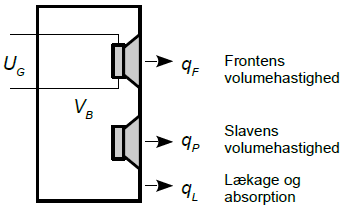
\includegraphics[width=0.5\linewidth]{graphics/57.png}
	\caption{Et kabinet med en passiv slave. \href{http://www.torean.dk/artikel/Elektroakustik.pdf}{(Elektroakustik, TAS)}}
	\label{fig:57}
\end{figure}

\begin{itemize}
	\item $M_{AS}=\dfrac{M_{MS}}{S_D^2}$
	\item $R_{AS}=\dfrac{R_{MS}}{S_D^2}$
	\item $C_{AS}=C_{MS}S_D^2$
\end{itemize}

\begin{itemize}
	\item Rød kurve er det resulterende lydtryk.
	\item Grøn kurve er	lydtrykket fra højttalerenheden.
	\item Blå kurve viser hvor meget slave står for.
\end{itemize}

\begin{figure} [H]
	\centering
	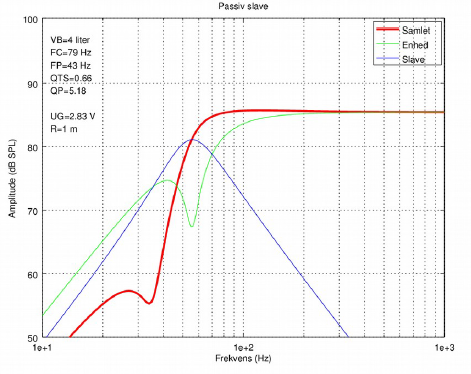
\includegraphics[width=0.75\linewidth]{graphics/61.png}
	\caption{basreflex kabinet. \href{http://www.torean.dk/artikel/Elektroakustik.pdf}{(Elektroakustik, TAS)}}
	\label{fig:61}
\end{figure}

\subsection{Øvelser}
\subsubsection{Øvelse 8.1}
Design et anden ordens delefilter for et tovejs system med en bas og diskanthøjttaler med udgangspunkt i formlerne fra noten \href{http://www.torean.dk/artikel/Elektroakustik.pdf}{Elektroakustik, s. 82}. Find et par højttalere på nettet og benyt de rapporterede frekvenskarakteristikker og øvrige data for de valgte enheder til at finde en egnet delefrekvens. \\

\noindent Beslut om diskanthøjttaleren skal ompoles (inverteres) eller forskydes mekanisk på fronten for at få en korrekt faserelation mellem enhederne. \\

\noindent Vælg godheden Q for hver gren af delefiltret. Beslut om der skal korrigeres for bashøjttalerens stigende impedans (s. 37) og for diskanthøjttalerens resonans, og beslut om diskanten skal dæmpes for at passe til bashøjttaleren (s. 85). Begrund de trufne valg!

